\chapter{Software OpenSource y Libre}
<<<<<<< HEAD
		\subsection{Deferencias} 
Una interpretación de lo que se entiende por el término \textit{open source}, cuando se utiliza en el contexto de la descripción de un programa de software o diseño de hardware, es que el código fuente del diseño se encuentra disponible a la vista de alguna forma. A pesar de que es una amplia y potencialmente término ambiguo , un común acuerdo sobre la definición está en un documento llamado la Open Source Definition (OSD ), publicado por la Open Source Initiative (OSI).
Una interpretación sencilla de lo que se entiende por el término open source , cuando se utiliza en el contexto de la descripción de un programa de software o diseño de hardware , es que el diseño Fuentes de alguna manera están disponibles a la vista. A pesar de que es un amplio y potencial término ambiguo, un común acuerdo sobre la definición está en un documento llamado  Open Source Definition (OSD ), publicado por la Open Source Initiative (OSI).

La definición no es una licencia de software libre en sí, si no algo para medir condiciones frente a la distribución para determinar si cumplen y, si lo hacen, entonces se puede decir que es \textit{open source}\cite{Etiqueta06}.La definición no es una licencia de software libre en sí, si no algo para medir condiciones frente a la distribución para determinar si cumplen y, si lo hacen, entonces se puede decir que es \textit{open source}. Cuando el software \textit{libre} o \textit{free} se utiliza para describir el software de código abierto, se refiere a los derechos y no al costo del usuario. La Fundación para el Software Libre (FSF) ofrece una definición para mostrar claramente qué se tiene que cumplir sobre el software para que pueda ser considerado libre \cite{Etiqueta07}. El termino Free Software Foundation (FOSS) es usado para referirse al software que se adhiere al OSD y FSF. El software libre y de código abierto es una sociedad inclusiva término que abarca tanto el software libre y software de código abierto que a pesar de describir modelos de desarrollo similares, tienen diferentes culturas y filosofías.

El software \textit{libre} se refiere a la libertad de los usuarios para ejecutar, copiar, distribuir, estudiar, cambiar y mejorar el software. El vocablo \textit{free} en ingles significa :gratis y/o libre. Por ello el término ha ocasionado confusiones dándose a entender, equivocadamente, que el software libre es gratuito o regalado. Pero no es una cuestión de presencia o ausencia de costo, puesto que el software libre no significa que no pueda ser comercial.

Stallman fundó la Free Software Foundation (FSF ) en 1985 para promover la libertad del usuario y para defender los derechos de todo el software libre( 28 ). La FSF patrocina el proyecto GNU. El software libre permite al usuario el ejercicio de cuatro libertades básicas:

\begin {itemize}
\item
 \textit{Libertad 0} Además el software \textit{libre} permite estudiar cómo funcionan y adaptarlo a las necesidades de quien lo use. Tener acceso a su código fuente posibilita, entre otras cosas, descubrir qué posibilidades tiene, etc. El adaptar el programa a las necesidades del usuario se puede suprimir partes que no le interesen, agregar otras partes que considere importantesm copiar una parte que realiza una tarea y/o adicinarla a otro programa, etc.

\item
\textit{Libertad 1} El software, sus copias y las modificaciones se pueden distribuir libremente, lo que significa poseer la libertad de redistribuir el programa, gratis o con algún costo, ya sea por mail, FTP, o en CD, redistibuyéndolo a una persona o a varias, a una persona que vive en otro país, etc.

\item 
\textit{Libertad 2} Es posible mejorarlo y hacer pública esas mejoras. La libretad de hacer un programa mejor, implica que se puede hacer menores los requerimientos de hardware para funcionar, que tenga mayores prestaciones, que sus requerimientos no sean tan altos, que tenga menos errores, etc. El poder liberar las mejoras al público quiere decir que si se realiza una mejora que permita un requerimiento menor de hardware, o que haga que ocupe menos espacio, se puede redistribuir ese programa mejorando o simplenete propoenr la mejora en lugar público (un foro de noticias, una lista de correo, un sitio web, un FTP, un canal de chat).

\item 
\textit{Libertad 3} El usuario al poseer el código fuente tiene poder de decisón, ya que podrá elegir quién puede modifica los programas que ha adquirido para mejorarlos (o bien mejorarlos el mismo). Es decir esto permite que no exista un monopolio, porque en el caso de que un software sea discontinuado el usuario podrá nuevamente (al poseer el código) elegir a un desarrollador para continuar utilizando el software que fue discontinuado. Además el usuario no estará completamente a merced de tener que renovar su hardware y software constantemente según ocurre a menudo con las políticas de las empresas que producen software privativo y también será libre de vender o redistribuir software libre.
 
 \end {itemize}
 
Mediante la licencias un autor permite el uso de su creación a otras personas, de la manera que el cree aceptable. En ese sentido la licencia es el instrumento que regula las maneras en que el usuario puede utilizar el software.

También una licencia de software es un contrato que determina en qué condiciones el usuario puede utilizar el programa informático y qué obligaciones asquiere para su uso. Cuando se instala un programa informático, o a veces, incluso, por el simple hecho de abrir el sobre que lo contiene, se esta aceptando las condiciones de su licencia de software.

Cuando IBM comenzó la venta de computadoras a gran escala en la década de 1960, el software venia incluido como código fuente. Una década más tarde, sin embargo, comenzaron a "desagregar"  el software, y se convirtió en habitual para los fabricantes de computadoras, no solo limito  el uso del mismo código fuente a los competidores, sino que también elimino la capacidad de modificar el código libremente y compartirlo%\cita{}(26).  
	
La licencia División de Software de Berkeley (BSD) y la Pública General del proyecto GNU (GNU GPL) son dos de las primeras licencias de código abierto. Ambos proporcionan la libertad de usar software de código fuente abierto para cualquier propósito y permitir la modificación y la distribución de su código fuente sin tener que pagar regalías. Las diferencias entre los dos pone de relieve una diferencia ideológica entre los defensores del código abierto .

Un punto significativo de diferencia entre las licencias BSD y GPL es que este último le permite
\textit{modificar su copia o copias del Programa o cualquier parte de el, y copie
y distribuir tales modificaciones ... supuesto que además ... hace que la
totalidad de cualquier trabajo que distribuya o publique y que en todo o en
parte contenga el Programa o cualquier parte del mismo, ya sea con o sin
modificaciones, para ser autorizadas sin cargo alguno para terceras partes bajo el
términos de esta Licencia Pública General.(GPLv1) ( 29 ). } %\cita{}

La GNU GPL se conoce como una licencia \textit{viral}, en que cualquier diseño haciendo uso de código ya licenciado bajo la GNU GPL debe ser entonces licenciado bajo la
GNU GPL o cualquier licencia juzgados como igualmente sin restricciones por la FSF. En pocas palabras, una condición de uso del código licenciado bajo GPL es que su diseño se debe tener licencia bajo la GPL o una licencia compatible. Las licencias que se consideran compatibles con la GPL por la FSF son generalmente similares en las libertades que garantiza el software libres. La licencia se transmite al código que hacen uso de ella. El GNU GPLv3 exige que cuando un proyecto adopta esta licencia el código fuente debe estar disponible y que las patentes o derechos digitales (DRM) no inhiben a otros del uso del diseño. 

La licencia BSD modificada es básicamente la misma que la original sin la clausula de publicidad. De acuerdo con dicha cláusula, todo el material de publicidad en el cual se menciona características o la utilización de este software tenia que mostrar el siguiente asentimiento:"este producto incluye software desarrollado por la Universidad de California, Berkeley y sus contribuyentes ".

Esta cláusula de publicidad no permitía que fuera compatible con la lincencia GPL pero a partir de su versión 2.0 fue eliminada y la licencia pasó a ser compatible con la GPL.

La GNU GPL es en cierto modo, más restrictiva que la licencia BSD sobre las libertad de hacer lo que uno quiere con el código fuente. En la GNU se estipula que el código modificado debe estar disponible, y cualquier diseño utilizado con código GPL tiene también que venir bajo la GNU GPL. Sin embargo, esto no es diferente a cualquier licencia comercial, donde el código fuente escrito por un empleado de una empresa,o todo el código que se modifican o crean esta bajo la licencia exclusiva de la empresa. En el caso de la licencia de GNU, sin embargo, los usuarios están obligados a mantener su diseño abierto y libre como la GPL de GNU hace, de la misma manera el empleado de la empresa está obligado a mantener su código propietario en secreto para cualquiera que no sea de la  empresa.

Otro punto de controversia es el uso combinado de los diseños en los que cada uno esta bajo una licencia diferente, dando lugar al concepto de \textit{compatibilidad de la licencia}. En el caso de que un diseño utilizara una librería bajo licencia GPL, la GNU GPL especifica que se puede utilizar si el diseño  que requiere la librería este también bajo la GPL. 

 Una solución para aquellos que deseen escribir bibliotecas, y no tienen la
interpretación más estricta de la trabajos derivados se les aplica la propuesta de el  Proyecto GNU la Licencia Pública General Reducida de GNU, o más conocida por su nombre en inglés GNU Lesser General Public License (antes GNU Library General Public License o Licencia Pública General para Bibliotecas de GNU),o simplemente por su acrónimo del inglés GNU LGPL, esta licencia permisiva se aplica a cualquier programa o trabajo que contenga una nota puesta por el propietario de los derechos del trabajo estableciendo que su trabajo puede ser distribuido bajo los términos de esta "LGPL Lesser General Public License". El "Programa", utilizado en lo subsecuente, se refiere a cualquier programa o trabajo original, y el "trabajo basado en el Programa" significa ya sea el programa o cualquier trabajo derivado del mismo bajo la ley de derechos de autor: es decir, un trabajo que contenga el Programa o alguna porción de él, ya sea íntegra o con modificaciones o traducciones a otros idiomas.
Otras actividades que no sean copia, distribución o modificación no están cubiertas en esta licencia y están fuera de su alcance. El acto de ejecutar el programa no está restringido, y la salida de información del programa está cubierta sólo si su contenido constituye un trabajo basado en el Programa (es independiente de si fue resultado de ejecutar el programa). Si esto es cierto o no depende de la función del programa.%\cita{wiki}

Estas diferencias de opinión con respecto a lo que constituye una obra derivada, y
la ambigüedad en torno a otros aspectos de la concesión de licencias de código abierto podría tener consecuencias para campos como el diseño de hardware y se discutirá en una sección posterior.

La principal diferencia de opinión, sin embargo , se deriva del hecho de que la libre
Software Foundation desean hacer imposible que el software propietario  pueda utilizar
software liberado bajo la GNU GPL. La FSF argumenta  que los que no están dispuesto a permitir que otras personas vean o modificar libremente su código aprovechen de los que si lo permiten. Otras licencias de código abierto, sin embargo ,son más permisivas en la utilización de sus diseños como por ejemplo en el codigo fuente de las librerias, en aplicaciones propietarias.

El objetivo del Proyecto GNU de implementar un sistema operativo completamente libre y gratuito, avanzo a buen ritmo en la década del 90, pero le faltaba la lleve de componentes del nivel más bajo.

El núcleo Linux iniciado por Linus Torvalds, fue liberado para poder ser modificado libremente en 1991. La licencia inicial, no fue exactamente una licencia d software libre, sin embargo la version 0.12 lanzada en febrero de 1992, fue licenciada nuevamente por Torvalds bajo los términos de la licencia pública general de GNU. Así como Unix en su tiempo, el núcleo de Torvalds atrajo la atención de programadores voluntario.

Hasta este punto, la falta de núcleo del proyecto GNU significaba la no existencia de un sistema operativo libre completo. El desarrollo de núcleo de Linux Torvalds lleno este último hueco. La conbinación del casi terminado sistema operativo GNU y el núcleo LInux resultó en el primer sistema operativo completo de softwore libre.

Entre las distribuciones Linux, Debian GNU/Linux, iniciada por Ian Murdock en 1993, es notorio por estar comprometido explicitamente con los prinicipios de GNU y la FSF del softwore libre. Los principios de desarrolladores de Debian estan expresados en el contrato social de Debian. Desde sus inicios, el proyecto de Debian ha estado intimamente ligado con la FSF, y de hecho fue patrocinado por la FSF durante un año. Sin embargo Debian ya no se considera software libre por la FSF y el proyecto GNU ya que el núcleo Linux incluido con Debian contiene partes privativas ademas de ofrecer repositorios con software no libre (18).

El GNU/Linux (o simplemente Linux) continúa siendo software libre desarrollado por programadores voluntarios, pero también muchas compañías ofrecen productos personalizados basados en el núcleo Linux así como distribuciones con soporte comercial.

El nombre del sistema operativo continúa generando controversias dentro de la comunidad de software libre, por un lado el proyecto GNU y otros grupos de usuarios piden que el sistema sea llamado GNU/Linux argumentando que la mayoría de los sistemas basados en el nucleo del Linux son derivaciones del sistema operativo GNU, que empezaron a desarrollarlos 7 años antes que el Linux Torvalds publicara su núcleo (19). Por otro lado, los grupos que apoyan el nombre Linux para referirse al sistema operativo completo y no solo a su núcleo, argumentan que el nombre Linux es mas reconocido, mejor recibido y mas practico (20). Es importante señalar que las mayorias de versiones de sistemas operativos basados en Linux, contienen muchas otras partes además que las desarrolladas por el proyecto GNU y el núcleo Linux, el ejemplo más representativo de estos componentes ajenos a GNU.

Ejemplos de otros exitosos y ampliamente adoptado proyectos de código abierto son el servidor web Apache , la oficina de los servicios públicos paquete OpenOffice.org y el proyecto Mozilla, que crea software de correo electrónico y navegador web. A pesar de que esta última pareja no eran originalmente de código abierto, el lanzamiento de su código fuente bajo licencias de código abierto fue significativa, y continúan los proyectos populares de la actualidad.

Tras la adopción creciente de software de código abierto en la década del 90, una organización llamada la \textit{Open Source Initiative} (OSI) fue iniciado por algunos los desarrolladores de software que se propusieron convencer a la gente que el software libre (como lo fue comúnmente conocida en ese entonces) tenía un lugar en la industria comercial. El éxito del modelo sorprendió a mucha personas, y demostró que era un modelo de desarrollo viable.  

A medida que la popularidad y la utilidad de Internet fue creciendo, también lo hicieron las  comunidades de codigo abierto por diferentes causas. La atracción y la comunicación que produce internet en personas interesadas en el desarrollo de código abierto proporcionan la chispa para las grandes comunidades de código abierto. Lo que ha dado como resultado un sinnúmero de comunidades y  grupos que contribuyen a el desarrollo de código fuente abierto de casi cualquier cosa.

Un sitio web, con sus comienzos en el año 2000, llamado OpenCores que proporcionar un sitio para la comunidad de hardware de código abierto. Fue una de las primeras comunidades de desarrollo de hardware y actualmente la mas grande, con más de cien mil usuarios y cerca de mil proyectos. Donde su principal objetivo es diseñar y publicar diseños de núcleo bajo una licencia de hardware siguiendo el modelo de la Licencia LGPL para el software. Estan comprometidos con el ideal de libre disposición, de libre uso y hardware de código abierto reutilizable.%\cita{}www.opencore

\subsection{OpenSource}

Dentro del software de código abierto se tiene alternativas como software multimedia avanzada, de productividad de oficina,  herramientas de gráficos, sistemas operativos y software de comunicaciones, por lo general libre para descargar y utilizar. Los gobiernos y las grandes empresas están aprovechando cada vez más el software de código abierto que existe y se están convirtiendo en importantes contribuyentes a los proyectos del software que adoptan. Las tendencias recientes han hecho mucho para disipar la imagen de la legión de solitarios desarrolladores de código abierto que son los únicos contribuyentes de trabajo. 
Como las entidades comerciales están aumentan la adopción y utilización de los proyectos de software libre,  se están convirtiendo en los contribuyentes más frecuentes. El kernel de Linux tiene ahora la mayor proporción de sus contribuciones de código de las entidades comerciales, ya sea por que están trabajando con el núcleo Linux en sus productos, o que deseen asegurar el apoyo a su hardware en el kernel, tales como Intel , AMD e IBM. Lo mismo es cierto para proyectos como Apache y MySQL.

La gran cantidad de software de código abierto disponible que existe ofrece la elección entre la adopción de software libre , pero con el lanzamiento de su obra derivada, y el desarrollo de una solución interna o la compra de una solución propietaria y revelando el trabajo no uno .		



		\subsection{¿Quien tiene el Hardware?}

		\subsection{OpenRISC}



%\cite{Etiqueta02},
%\textit{FPGAs}) .
%\begin {itemize}
%\item  Bloques lógicos configurables y \textit{Lookup Tables}.
% \end {itemize}

\begin{figure}[h!]
 \begin{center}
  % 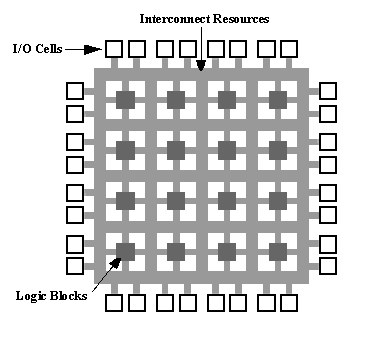
\includegraphics[width=0.5\textwidth,keepaspectratio=true]{./images/fpga1a}
 % \caption{Componentes de una FPGA}
  \label{fig:esquema}
 \end{center}
\end{figure}

<<<<<<< HEAD

%Conclusión!!Trabajar con un sistema final bajo licencias de hardware siguiendo el modelo de la Licencia LGPL para el software. Estamos comprometidos con el ideal de libre disposición, de libre uso y hardware de código abierto reutilizable.

=======

